All further reservoirs were constructed with the parameters from this baseline,
unless otherwise specified. The default reservoir size used was 200 hidden
nodes. $\mathbf{W}^{res}$ and $\mathbf{W}^{in}$ were both generated as random
matrices with i.i.d. entries in the interval [-0.5, 0.5]. Both matrices are
fully connected, and the reservoir weight matrix was rescaled such that
$\rho(\mathbf{W}_{res}) = 0.9$. The first 200 states of each run are discarded
to provide a \textit{washout} of the initial reservoir state. For all
experiments, the generated input was split into a training and test set, with
$L_{train} = 2000$ and $L_{test} = 3000$. All reported performances are the mean
across ten randomizations of each model representative. The Python software
library implementation is available online\footnote{Some GitHub repository.}.

\subsection{Noise}

We model AWGN by extending the ESN model to take the sum of two individual
inputs, $\mathbf{u}(t)$ and $\mathbf{v}(t)$, which represent the signal and the
noise. The goal of the reservoir remains a computation on the signal
$\mathbf{u}(t)$, a task now hindered by the unwanted noise.

We vary the signal to noise ratio of the injected noise when running the test
dataset. The signal to noise ratio is measured in dB, and is calculated as $SNR
= 10\log_{10}(\frac{var(u)}{var(v)})$. The results are shown in
Fig. \ref{input_noise_snr}, illustrating a slight performance degradation when
the ratio of signal power to noise power drops below 20 dB. The reservoir
performance drops more drastically when reaching 10 dB. Similar performance
degradation was seen in \cite{dambre_information_2012}, where the same SNR
measure was used to evaluate the signal reconstruction capacity from the state
of a dynamical system.

\begin{figure}
  \centering
  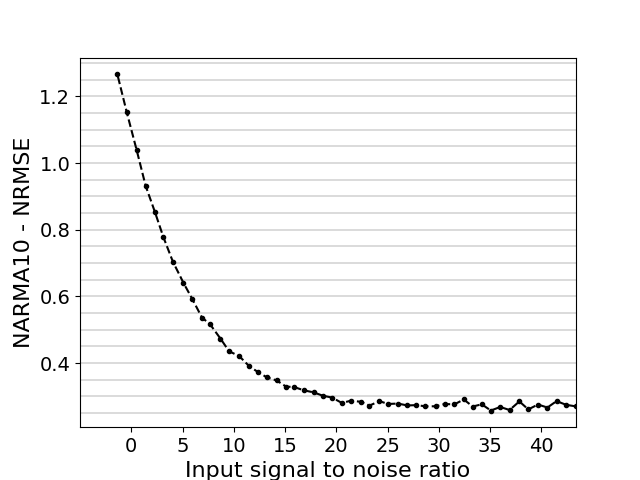
\includegraphics[width=2.5in]{img/input_noise_snr.png}
  \caption{
    Noise causing a decrease in performance for an ESN reservoir on the NARMA10
task ($N = 200$ nodes).
  }
  \label{input_noise_snr}
\end{figure}

\subsection{Measurement equipment accuracy}

To emulate the behavior of an ADC, we extend our ESN model to allow for
quantization of reservoir output before it is passed to the readout layer. This
quantization effectively divides the range of the nonlinear activation function
of each hidden node into a discrete set of fixed output bins.

\begin{figure}[H]
  \centering
  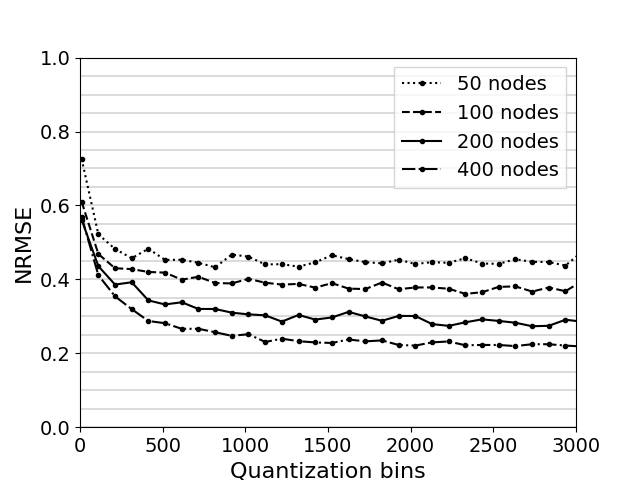
\includegraphics[width=2.5in]{img/adc_quantization.png}
  \caption{
    Performance effect of ADC quantization on four reservoirs of different
sizes. $\tanh$ is used as activation function for the experiment, dividing its
range of (1-, 1) into $n$ discrete output bins.
  }
  \label{adc_quantization}
\end{figure}

% (TODO): Change this to bits of quantization? As if it's an actual ADC.

Fig. \ref{adc_quantization} shows how quantization affects reservoir
performance. We plot the error of four different reservoir sizes: 50, 100, 200
and 400 hidden nodes to see whether it is possible to compensate for lower
resolutions by increasing the size of the reservoir.

\subsection{Partially visible reservoir state}

We begin by experimenting with the sparsity of $\mathbf{W}_{in}$ and
$\mathbf{W}_{out}$. In both cases, we now generate the connection matrices such
that a wanted density, given as the fraction of connected nodes, is
achieved. Input and output is adjusted separately. Fig. \ref{partial_visibility}
shows the results of our simulation runs.

Additionally, we examine three different input weight distributions: uniform,
Gaussian and fixed. All inputs are all sampled as i.i.d streams. The uniform
distribution is sampled in the interval [-0.5, 0.5], the Gaussian distribution
is sampled with a zero mean and standard deviation $\sigma = 1.0$, and the fixed
distribution has every input weight set to 1. Moreover, we explore the parameter
space of the input scaling in the interval [0.1, 1.0].

%%% Local Variables:
%%% mode: latex
%%% TeX-master: "../main"
%%% End:
